\section{Evaluation Metrics}
\hspace{\parindent}
Evaluation metrics to assess the effectiveness of the anomaly detection and fraud identification process:

\begin{itemize}
	\item \textbf{Accuracy}: Measures the overall correctness of the predicted labels compared to the true labels.
	\item \textbf{Precision}: Indicates the proportion of correctly identified potentially fraudulent transactions among all transactions identified as potentially fraudulent.
	\item \textbf{Recall}: Represents the proportion of correctly identified potentially fraudulent transactions among all truly fraudulent transactions.
	\item \textbf{F1 Score}: Harmonic mean of precision and recall, providing a balance between the two metrics.
	\item \textbf{Confusion Matrix}: Provides a detailed breakdown of true positive, false positive, true negative, and false negative predictions.
\end{itemize}


\begin{table}[H]
	\centering
	\caption{Evaluation Metrics}
	\label{tab:results}
	\begin{tabular}{@{}ll@{}}
		\toprule
		Metric      & Value   \\ \midrule
		Accuracy    & 0.9803  \\
		Precision   & 0.0016  \\
		Recall      & 0.0223  \\
		F1 Score    & 0.0029  \\
		\bottomrule
	\end{tabular}
\end{table}

\begin{table}[H]
	\centering
	\caption{Confusion Matrix}
	\label{tab:confusion_matrix}
	\begin{tabular}{@{}cc|cc@{}}
		\toprule
		\multicolumn{2}{c|}{\textbf{}} & \multicolumn{2}{c}{\textbf{Predicted}} \\ \midrule
		\multicolumn{1}{c|}{}          &          & \textbf{Fraudulent}      & \textbf{Non-Fraudulent}    \\ \midrule
		\multicolumn{1}{c|}{\textbf{True}} & \textbf{Fraudulent} & 183                   & 8030                  \\
		\multicolumn{1}{c|}{\textbf{Labels}} & \textbf{Non-Fraudulent} & 117004                & 6237403               \\ \bottomrule
	\end{tabular}
\end{table}

\begin{figure}[H]
	\centering
	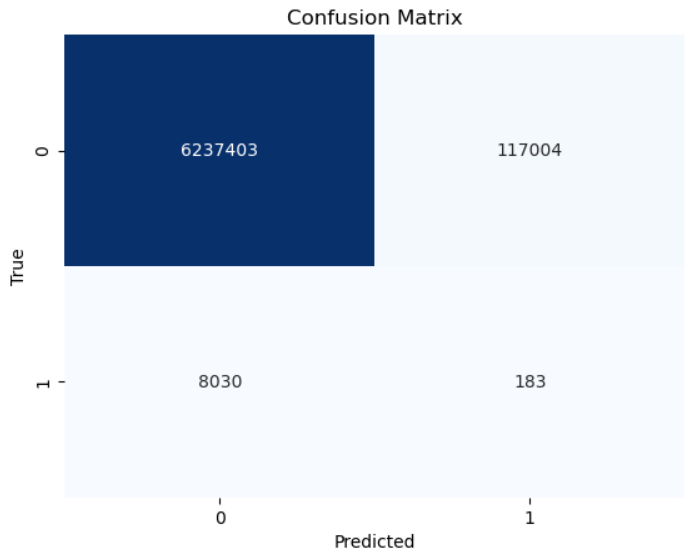
\includegraphics[width=0.7\linewidth]{chap4/6}
	\caption{Confusion Matrix}
	\label{fig:6}
\end{figure}


\begin{table}[htbp]
	\centering
	\caption{Classification Report}
	\label{tab:classification_report}
	\begin{tabular}{lcccc}
		\toprule
		\textbf{Class} & \textbf{Precision} & \textbf{Recall} & \textbf{F1-Score} & \textbf{Support} \\
		\midrule
		0 & 1.00 & 0.98 & 0.99 & 6354407 \\
		1 & 0.00 & 0.02 & 0.00 & 8213 \\
		\midrule
		\textbf{Accuracy} & \multicolumn{4}{c}{0.98} \\
		\textbf{Macro Avg} & 0.50 & 0.50 & 0.50 & 6362620 \\
		\textbf{Weighted Avg} & 1.00 & 0.98 & 0.99 & 6362620 \\
		\bottomrule
	\end{tabular}
\end{table}

\section{Receiver Operating Characteristic (ROC) Curve Analysis}
\hspace{\parindent}
Analyze the performance of the anomaly detection and fraud identification system using the Receiver Operating Characteristic (ROC) curve:

\begin{itemize}
	\item \textbf{ROC Curve:} Evaluate the model's ability to distinguish between true positive and false positive classifications across different threshold values. The curve plots the true positive rate (TPR) against the false positive rate (FPR), providing insights into the trade-off between sensitivity and specificity.
	
	\item \textbf{Area Under the Curve (AUC):} Calculate the Area Under the Curve (AUC) metric to quantify the overall performance of the ROC curve. A higher AUC value indicates better discrimination between positive and negative classes.
	
	\item \textbf{Visual Representation:} The ROC curve is visualized using a line plot, where the AUC value is displayed in the legend. Additionally, a diagonal reference line is included to represent random guessing.
\end{itemize}

\begin{figure}[H]
	\centering
	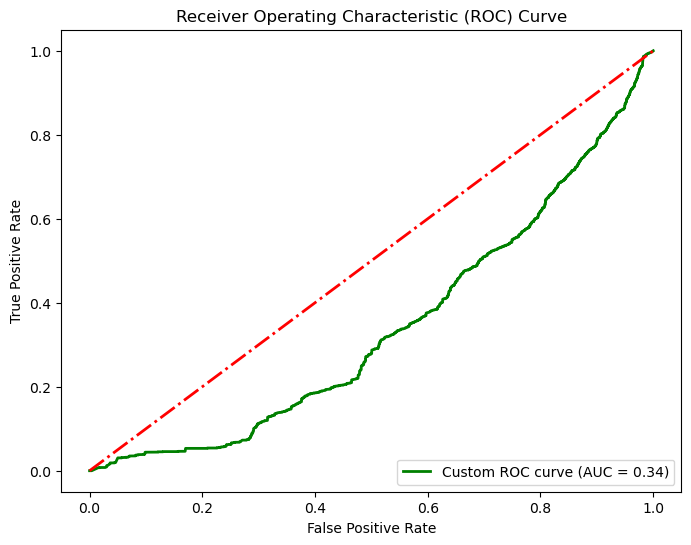
\includegraphics[width=0.7\linewidth]{chap4/7}
	\caption{ROC Analysis}
	\label{fig:7}
\end{figure}

\section{Development Directions}

\begin{itemize}
	\item \textbf{Feature Engineering:} Explore additional features that could enhance the detection of fraudulent transactions, such as transaction frequency, geographical location, or user behavior patterns.
	\item \textbf{Model Optimization:} Fine-tune hyperparameters and architecture of the Graph Neural Network (GNN) model to improve its performance in capturing subtle patterns indicative of fraud.
	
	\item \textbf{Ensemble Methods:} Investigate the use of ensemble methods, combining multiple models such as GNNs, Isolation Forests, and traditional machine learning algorithms, to leverage their complementary strengths.
	
	\item \textbf{Advanced Anomaly Detection Techniques:} Experiment with advanced anomaly detection techniques beyond Isolation Forest, such as autoencoders, one-class SVMs, or deep learning-based approaches, to further enhance detection accuracy.
	
	\item \textbf{Real-time Monitoring:} Develop mechanisms for real-time monitoring of transactions, enabling immediate detection and prevention of fraudulent activities as they occur.
\end{itemize}